\documentclass[12pt,letterpaper]{article}
% The usepackage tell LaTeX which packages are needed. As you get better you can add more
% packages for extra functionality
% Percent signs are comments, they will not be read by the renderer.
\usepackage{fullpage}
\usepackage[top=2cm, bottom=2.5cm, left=2.5cm, right=2.5cm]{geometry}
\usepackage{amsmath,amsthm,amsfonts,amssymb,amscd}
\usepackage{lastpage}
\usepackage{enumerate}
\usepackage{fancyhdr}
\usepackage{mathrsfs}
\usepackage{xcolor}
\usepackage{graphicx}
\usepackage{multicol}
\usepackage{wrapfig}
\usepackage{hyperref}
\usepackage{systeme}
\usepackage[shortlabels]{enumitem}
\usepackage{listings} %for listings of the source code

% Some definitions for using the listing package.
% When we reference 'codegreen', it will be the RGB color defined below.
\definecolor{codegreen}{rgb}{0,0.6,0}
\definecolor{codegray}{rgb}{0.5,0.5,0.5}
\definecolor{codepurple}{rgb}{0.58,0,0.82}
\definecolor{backcolour}{rgb}{0.95,0.95,0.92}
\DeclareUnicodeCharacter{2212}{-}

% Also for the listings, this will make the code listing look like default MATLAB
\lstdefinestyle{mystyle}{
	backgroundcolor=\color{backcolour},   
	commentstyle=\color{codegreen},
	keywordstyle=\color{magenta},
	numberstyle=\tiny\color{codegray},
	stringstyle=\color{codepurple},
	basicstyle=\footnotesize,
	breakatwhitespace=false,         
	breaklines=true,                 
	captionpos=b,                    
	keepspaces=true,                 
	numbers=left,                    
	numbersep=5pt,                  
	showspaces=false,                
	showstringspaces=false,
	showtabs=false,                  
	tabsize=2
}
\lstset{style=mystyle}

\hypersetup{%
  colorlinks=true,
  linkcolor=blue,
  linkbordercolor={0 0 1}
}
 
\setlength{\parindent}{0.0in}
\setlength{\parskip}{0.05in}

\newcommand\course{COMP 521}
\newcommand\hwnumber{5}             
\newcommand\MyName{Zack Humphries}  

\pagestyle{fancyplain}
\headheight 15pt
\lhead{\MyName}
%\lhead{\NetIDa\\\NetIDb}                 % <-- Comment this line out for problem sets (make sure you are person #1)
\chead{\textbf{\Large Homework \hwnumber}}
\rhead{\course\\ October 28, 2022}
\lfoot{}
\cfoot{}
\rfoot{\small\thepage}
\headsep 1.5em

\begin{document}

\newcommand{\norm}[1]{\left\lVert#1\right\rVert}

\section*{Problem 1}
Find the roots to the following functions $f(x)$.
\begin{enumerate}[label=(\alph*)]
	\item \label{f1} $f(x) = -x^2 +x + 2$,
	\item \label{f2} $f(x) = e^x -2 - x$,	
\end{enumerate}

using:

\begin{enumerate}
	\item \textbf{Fixed point iteration}. Choose your $g(x)$ and a tolerance of $10^{-9}$. For \ref{f1} start with the following points $p_0 =\{\,2.5\,;\,0.15\,;\,1.5\,\}$. For \ref{f2} start with the following points $p_0 =\{\,2.5\,; \,0.15\,;\, 0.25\,\}$. What can you say about the convergence? \textbf{Explain}.
	
    For the fixed point iteration, I chose my $g(x)$ to be\ldots
\begin{equation}
    g_{a}(x) = \pm \sqrt{x+2}
\end{equation}
\begin{equation}
    g_{b}(x) = e^{x}-2
\end{equation}
    for \ref{f1} and \ref{f2}, respectively. I chose $g_{a}(x) = \pm \sqrt{x+2}$ instead of\ldots
\begin{equation}
    g_{a}(x) = x^{2}-2
\end{equation}
    because $g_{a}(x) = x^{2}-2$ would not work for $p_{0} = 2.5$. Plugging the $p_{0}=2.5$ into $g'_{a}(x)=2x$ is $5$, would break the rule of fixed point iterations, where\ldots
\begin{equation}
    \left\lvert g'(x) \right\rvert  < k < 1 \hspace*{.2cm}\forall \hspace*{.2cm} x \in \left[a,b\right] 
\end{equation}
In most cases, using the negative of (1) would result in imaginary numbers, but given that Matlab extends its functionality into complex numbers, the function $g_{a}(x) = - \sqrt{x+2}$ works in the complex number space and $g'_{a}(x)$ is never larger than 1 for the given $p_{0}$s.


Another note is that since the $g_{b}(x) = e^{x}-2$, a $p_{0}=2.5$ would not work because plugging $p_{0}=2.5$ into $g'_{b}(x)=e^{x}$ is $e^{2.5}>1$ which breaks the rule of fixed point iterations.


The graphs of the convergence are plotted below. The fixed point iteration of $g_{a}(x)$ converges on both the roots, $x=2$ and $x=-1$, where as $g_{b}(x)$ only converges on one of the roots, $x=-1.84$
\pagebreak
\begin{figure}[!h]
    \centering
    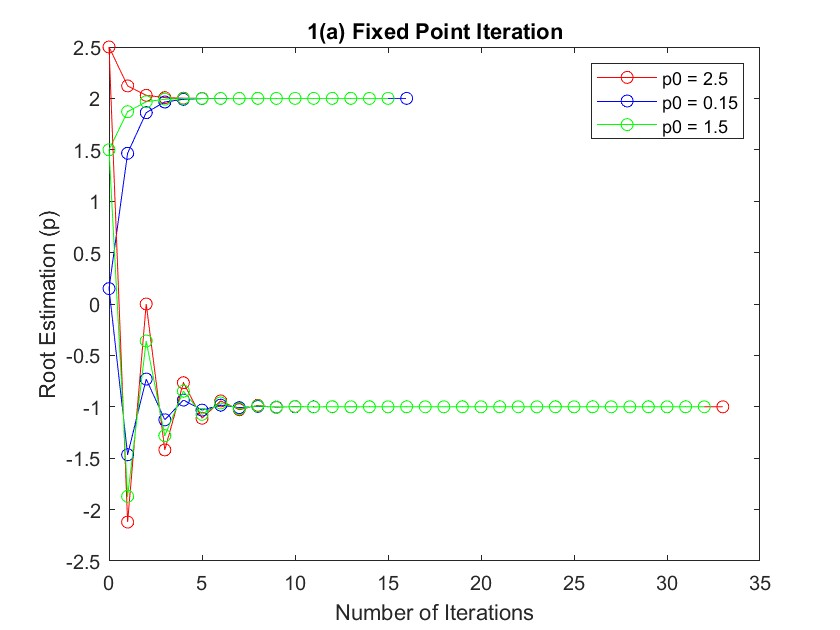
\includegraphics[width = 0.8\linewidth]{1a_fixed_iteration.jpg}
    \caption{1(a)\: Fixed Point Iteration}\label{fig:1a_fixed_iteration}
    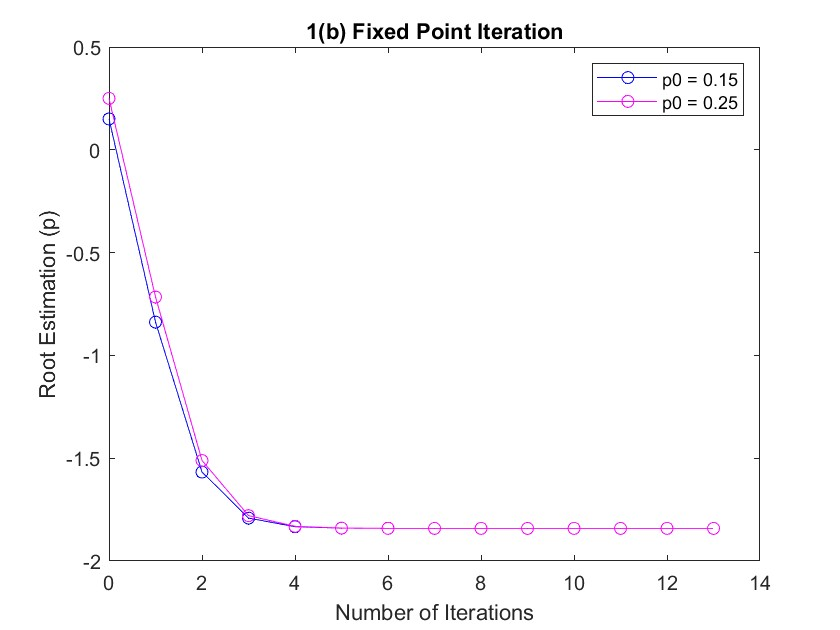
\includegraphics[width = 0.8\linewidth]{1b_fixed_iteration.jpg}
    \caption{1(b)\: Fixed Point Iteration}\label{fig:1b_fixed_iteration}
\end{figure}

\pagebreak


	\item \textbf{Bisection method}. Choose a tolerance of $10^{-9}$. For \ref{f1} and \ref{f2} use the intervals $x \in [\,-4.0\,;\,1.0\,]$ and $x \in [\,0.5\,;\,3.0\,]$. What can you say about the convergence? \textbf{Use plots and discuss}.


For the functions\ldots
\begin{equation}
    f_{a}(x) = -x^2 +x + 2
\end{equation}
\begin{equation}
    f_{b}(x) = e^x - x -2
\end{equation}

The roots are at $x =-1$, $x=2$ and $x\approx -1.84$, $x\approx 1.15$ respectively. 
Since we use the intervals $x \in [\,-4.0\,;\,1.0\,]$ and $x \in [\,0.5\,;\,3.0\,]$, these intervals are perfectly placed such that they are between the two roots in each equation.
Thus, they will converge on those roots as shown in figures 3 and 4.

    
\pagebreak
\begin{figure}[!h]
    \centering
    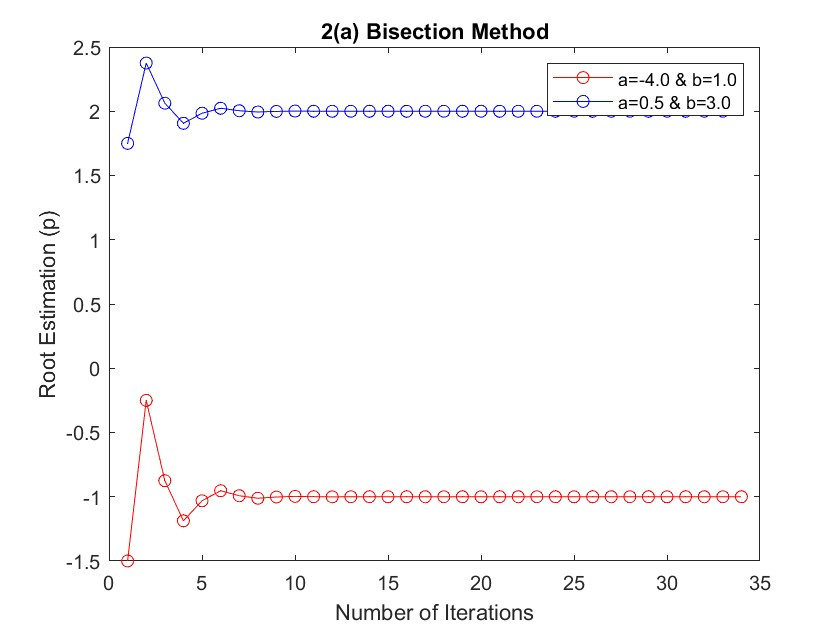
\includegraphics[width = 0.8\linewidth]{2a_bisection_method.jpg}
    \caption{2(a)\: Bisection Method}\label{fig:2a_bisection_method}
    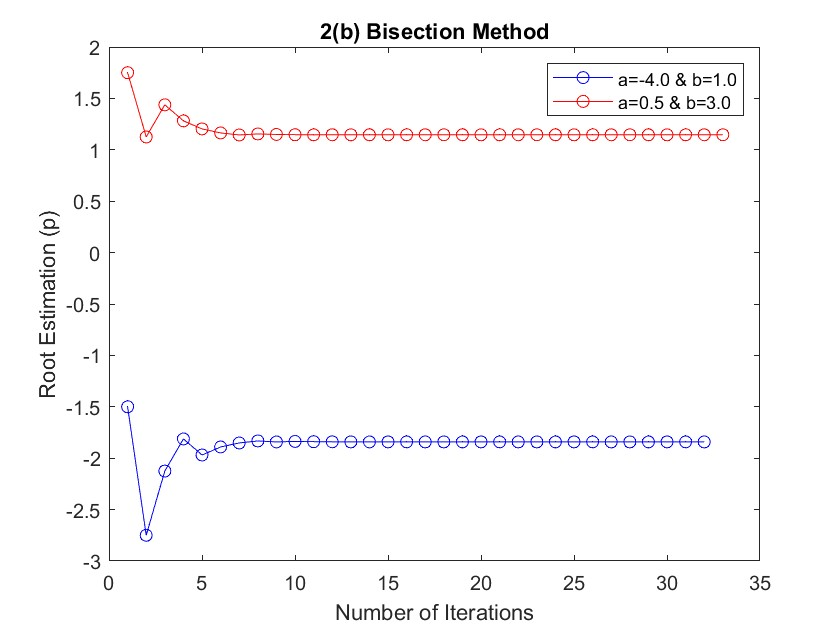
\includegraphics[width = 0.8\linewidth]{2b_bisection_method.jpg}
    \caption{2(b)\: Bisection Method}\label{fig:2b_bisection_method}
\end{figure}

\pagebreak



	\item \textbf{Newton's method}. Choose $\delta=\epsilon=10^{-9}$. For \ref{f1} and \ref{f2} start with the following points $p_0 =\{\,-3.0\,;\,0.0\,;\,6.0\,\}$. What can you say about the convergence? \textbf{Use plots and discuss}.
For the functions\ldots
\begin{equation}
    f_{a}(x) = -x^2 +x + 2
\end{equation}
\begin{equation}
    f_{b}(x) = e^x - x -2
\end{equation}

The points $p_{0} =\{\,-3.0\,;\,0.0\,;\,6.0\,\}$ all converge for $f_{a}(x)$ because none of the points are located at or very close to a local minimum or maximum where\ldots
\begin{equation}
    f'_{a}(x) = -2x + 1 = 0, \hspace*{0.5cm} x=0.5
\end{equation}
However, for $f_{b}(x)$, the point $p_{0}=0.0$ does not converge because $x=0.0$ is located at a local minimum where\ldots
\begin{equation}
    f'_{b}(x) = e^x - 1 = 0, \hspace*{0.5cm} x=0.0
\end{equation}
thus, it is omitted from figure 6 below.

\pagebreak
\begin{figure}[!h]
    \centering
    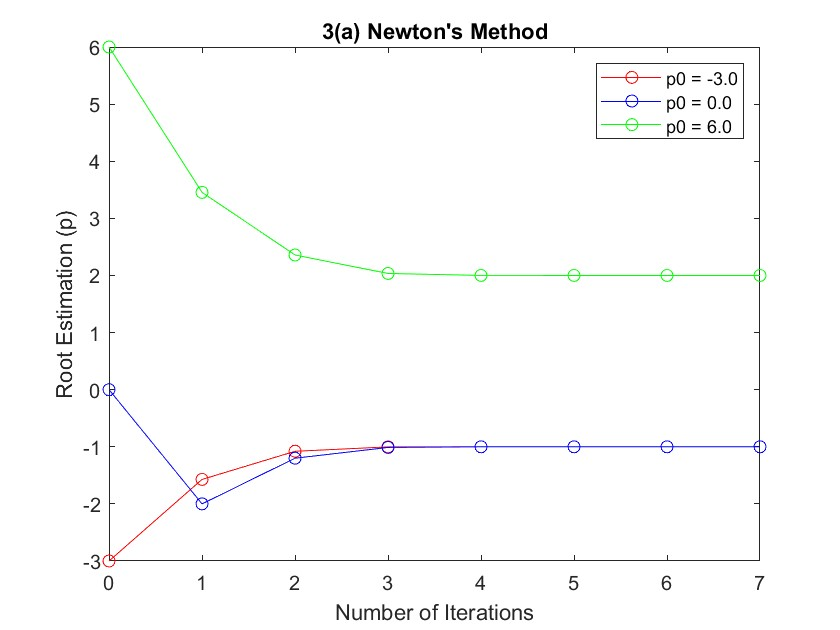
\includegraphics[width = 0.8\linewidth]{3a_newtons_method.jpg}
    \caption{2(a)\: Newton's Method}\label{fig:3a_newtons_method}
    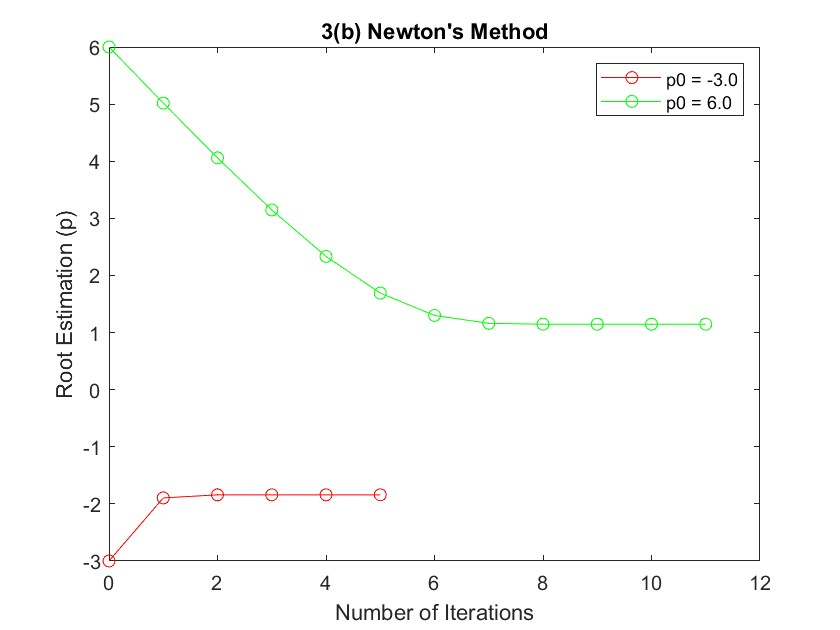
\includegraphics[width = 0.8\linewidth]{3b_newtons_method.jpg}
    \caption{2(b)\: Newton's Method}\label{fig:3b_newtons_method}
\end{figure}

\end{enumerate}

\pagebreak

\lstset{title={fixed\_point\_iteration.m}}
\begin{lstlisting}[language = Matlab]
function [root, iteration, guess_list] = fixed_point_iteration(g, tolerance, guess)
    x0 = guess;
    flag = true;
    iteration = 0;
    max_iterations = 1000;
    guess_list = [guess];

    while (flag || (iteration<max_iterations))
        x = g(x0);
        if(abs(x-x0)<tolerance)
            flag = false;
            root = x;
            break
        end
        x0=x;
        guess_list = [guess_list, x0];
        iteration = iteration + 1;
    end
end
\end{lstlisting}
\pagebreak
\lstset{title={bisection\_method.m}}
\begin{lstlisting}[language = Matlab]
function [root, iterations, guess_list] = bisection_method(f, a,b, tolerance)
    iterations = 0;
    tol = 1;
    if ( f(a) == 0 )
        root = a;
        return;
    elseif ( f(b) == 0 )
        root = b;
        return;
    elseif ( f(a) * f(b) > 0 )
        fprintf('f(a) and f(b) do not have opposite signs');
        return;
    end

    guess_list=[];

    while (tol>tolerance)
        iterations = iterations+1;
        mid=(a+b)/2;
        fa=f(a);
        fb=f(b);
        fmid=f(mid);
        guess_list = [guess_list, mid];

        if (fa*fmid < 0)
            b=mid;
            tol = abs(fa-fmid);
        elseif (fb*fmid <0)
            a=mid;
            tol = abs(fb-fmid);
        elseif (fmid==0)
            root = mid;
            tol=0;
        else
            fprintf('f(a), f(b), and f(mid) all have the same sign\n');
            root = "N/A";
            return;
        end
        root = mid;
    end  
end

\end{lstlisting}
\pagebreak
\lstset{title={newtons\_method.m}}
\begin{lstlisting}[language = Matlab]
function [root, iterations, guess_list] = newtons_method(f, fprime, guess1, delta)
    iterations = 0;
    tol=1;
    guess = guess1;
    guess_list = [guess];
    while (tol>delta || abs(f(guess))>delta)
        iterations = iterations+1;
        x = guess;
        prime = fprime(x);
        guess = x-(f(x)/prime);
        if (isnan(guess)|| isinf(guess))
            fprintf("x=%.2f is or is near a local maximum or minimum so results in an error\n",guess1)
            root = "N/A";
            return;
        end
        guess_list = [guess_list, guess];
        tol = abs(f(guess)-f(x));
    end
    root=guess;
end
\end{lstlisting}
\pagebreak
\lstset{title={main.m}}
\begin{lstlisting}[language = Matlab]
%% Zack Humphries
% COMP 521
% HW5

clc;       % clear command window
clear;     % removes all saved variables
close all; % close any open windows


%% 1(a)
ga = @(x) (x+2)^(1/2);
tol = 10^(-9);

p0 = [2.5 0.15 1.5];
plot_color_setting = ["-or", "-ob", "-og"];
fprintf("Fixed Point Iteration:\n")
fprintf("a)\n")
for n=1:3
    [root, iterations, guess_list] = fixed_point_iteration(ga, tol, p0(n));
    fprintf("With p0=%.2f, the root is %.2f and it took %i iterations to find the root\n", p0(n), root, iterations)
    plot([0:1:iterations], guess_list, plot_color_setting(n))
    hold on
end

ga = @(x) -(x+2)^(1/2);
for n=1:3
    [root, iterations, guess_list] = fixed_point_iteration(ga, tol, p0(n));
    fprintf("With p0=%.2f, the root is %.2f and it took %i iterations to find the root\n", p0(n), root, iterations)
    plot([0:1:iterations], guess_list, plot_color_setting(n))
    hold on
end
title("1(a) Fixed Point Iteration")
xlabel("Number of Iterations")
ylabel("Root Estimation (p)")
legend("p0 = 2.5", "p0 = 0.15", "p0 = 1.5")
fprintf("\n")
hold off


% 1(b)
gb = @(x) exp(x)-2;
plot_color_setting = ["-ob", "-om"];
fprintf("b)\n")
figure(2)
p0 = [0.15 0.25]; % 2.5 doesn't work
for n=1:2
    [root, iterations, guess_list] = fixed_point_iteration(gb, tol, p0(n));
    fprintf("With p0=%.2f, the root is %.2f and it took %i iterations to find the root\n", p0(n), root, iterations)
    plot([0:1:iterations], guess_list, plot_color_setting(n))
    hold on
end
title("1(b) Fixed Point Iteration")
xlabel("Number of Iterations")
ylabel("Root Estimation (p)")
legend("p0 = 0.15", "p0 = 0.25")
fprintf("\n")
hold off

%% 2(a)
fa = @(x) -(x^2)+x+2;
fb = @(x) exp(x)-x-2;
figure(3)

range1 = [-4.0 1.0];
range2 = [0.5 3.0];
fprintf("Bisection Method:\n")
fprintf("a)\n")
[root, iterations, guess_list] = bisection_method(fa, range1(1),range1(2), tol);
plot([1:1:iterations], guess_list, '-or')
fprintf("With a=%.2f and b=%.2f, the root is %.2f and it took %i iterations to find the root\n", range1(1), range1(2), root, iterations)
hold on
[root, iterations, guess_list] = bisection_method(fa, range2(1),range2(2), tol);
plot([1:1:iterations], guess_list, '-ob')
fprintf("With a=%.2f and b=%.2f, the root is %.2f and it took %i iterations to find the root\n", range2(1), range2(2), root, iterations)
fprintf("\n")
title("2(a) Bisection Method")
xlabel("Number of Iterations")
ylabel("Root Estimation (p)")
legend("a=-4.0 & b=1.0", "a=0.5 & b=3.0")
hold off

%2(b)
figure(4)
fprintf("b)\n")
[root, iterations, guess_list] = bisection_method(fb, range1(1),range1(2), tol);
plot([1:1:iterations], guess_list, '-ob')
fprintf("With a=%.2f and b=%.2f, the root is %.2f and it took %i iterations to find the root\n", range1(1), range1(2), root, iterations)
hold on
[root, iterations, guess_list] = bisection_method(fb, range2(1),range2(2), tol);
plot([1:1:iterations], guess_list, '-or')
fprintf("With a=%.2f and b=%.2f, the root is %.2f and it took %i iterations to find the root\n", range2(1), range2(2), root, iterations)
fprintf("\n")
title("2(b) Bisection Method")
xlabel("Number of Iterations")
ylabel("Root Estimation (p)")
legend("a=-4.0 & b=1.0", "a=0.5 & b=3.0")
hold off


%% 3(a)
fprimea = @(x) -2*x+1;
fprimeb = @(x) exp(x)-1;
figure(5)

p0 = [-3.0 0.0 6.0];
plot_color_setting = ["-or", "-ob", "-og"];
fprintf("Newton's Method:\n")
fprintf("a)\n")
for n=1:3
    [root, iterations, guess_list] = newtons_method(fa, fprimea, p0(n), tol);
    plot([0:1:iterations], guess_list, plot_color_setting(n))
    hold on
    fprintf("With p0=%.2f, the root is %.2f and it took %i iterations to find the root\n", p0(n), root, iterations)
end
fprintf("\n")
title("3(a) Newton's Method")
xlabel("Number of Iterations")
ylabel("Root Estimation (p)")
legend("p0 = -3.0", "p0 = 0.0", "p0 = 6.0")
fprintf("\n")
hold off

% 3(b)
fprintf("b)\n")
figure(6)
for n=1:3
    [root, iterations, guess_list] = newtons_method(fb, fprimeb, p0(n), tol);
    if (isnumeric(root))
        plot([0:1:iterations], guess_list, plot_color_setting(n))
        hold on
    end
    fprintf("With p0=%.2f, the root is %.2f and it took %i iterations to find the root\n", p0(n), root, iterations)
end
fprintf("\n")
fprintf("\n")
title("3(b) Newton's Method")
xlabel("Number of Iterations")
ylabel("Root Estimation (p)")
legend("p0 = -3.0", "p0 = 6.0")
\end{lstlisting}    




\end{document}